\documentclass[a4paper]{article}

\usepackage[english]{babel}
\usepackage[utf8]{inputenc}
\usepackage{amsmath}
\usepackage{graphicx}
\usepackage{color}
\usepackage{geometry}
\usepackage[colorinlistoftodos]{todonotes}

\title{Report Practical assignment 1}

\author{TheMachinists team:\vspace{0.5cm}\\
Fares Ben Slimane \\
Parviz Haggi \\
Mohammed Loukili \\
Jorge A. Gutierrez Ortega
}

\date{\today}

\begin{document}
\maketitle

\begin{abstract}
This report explains our approaches to solving the problems of the practical assignment~1, the experiments we performed, the results and conclusion of our work. The code we developped is uploaded to our Github repository \cite{github}
\end{abstract}

\section{Problem 1 (MLP)}
\label{sec:problem1}

\subsection{Building model}

\begin{enumerate}
  \item Using the python script mlp.py under the folder problem~1  \cite{github}, we built an MLP with two hidden layers h1 (512 hidden units), and h2 (256 hidden units).The total number of the parameters of this network is: 
  $$ 784*512 + 512 + 512*256 + 256 + 256*10 + 10 = 535,818 \approx 0.5 M$$
  
  \item We implemented the forward and backward propagation for a flexible network that can include  any number of layers. This was done with the numpy package follwing the provided class structure and without the use of deep learning framework. (See python script mlp.py under problem 1 folder).
  
  \item We trained the MLP using cross entropy as the training criterion (See loss method in the NN class in the mlp.py script) which is then minimized in order to find the optimal model parameters. To this end we used  stochastic gradient descent (See the update method in the NN class in the mlp.py script). 
  
\end{enumerate}

\subsection{Initialization}
We consider a model architecture of two hidden layers h1  with 512 hidden units and h2  with 256 hidden units, and a total number of 535,818 parameters. We chose RELU as an activation function, a learning rate of 0.01 and a mini-batch size of 64.
\begin{enumerate}
  \item We trained the model for 10 epochs using the 3 initialization methods (Zero, normal and glorot) and we recorded the average
loss measured for each method.

\begin{itemize}
  \item Zero initialization(Figure 1): 2.3, 2.3, 2.3, 2.3, 2.3, 2.3, 2.3, 2.3, 2.3, 2.3
  \item Normal initialization(Figure 2): inf, inf, 4.37, 2.90, 2.15, 1.67, 1.35, 1.11, 0.94, 0.80
  \item Glorot initialization(Figure 3): 0.85, 0.36, 0.30, 0.27, 0.24, 0.22, 0.21, 0.19, 0.18, 0.17
\end{itemize}

\item We plot the losses against the training time (epoch) using each initialization method (Figures \ref{fig:init1}, \ref{fig:init2} and \ref{fig:init3}). We conclude from the plots that the glorot initialization is the best among the methods in which the loss decreases rapidly at each epoch whereas, for the zero initialization, the loss decreases very slowly. An explanation for this is that by initializing all the weights to zero, all the hidden nodes will have the same value and the network will learn just one function. This is called the symmetry problem, which is dealt with by initializing the weights randomly (as in the cases of Glorot and normal initializations)\cite{weights}.

\end{enumerate}


\begin{figure}
\centering
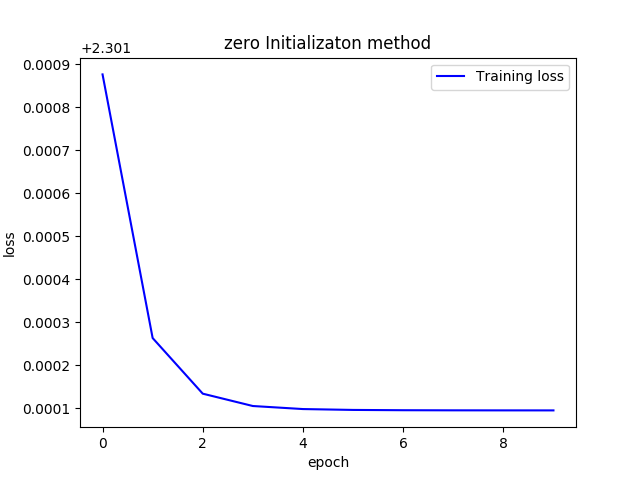
\includegraphics[width=0.7\textwidth]{zero_init.png}
\caption{\label{fig:init1}average loss against the training time (epoch) using zero initialization method.}
\end{figure}

\begin{figure}
\centering
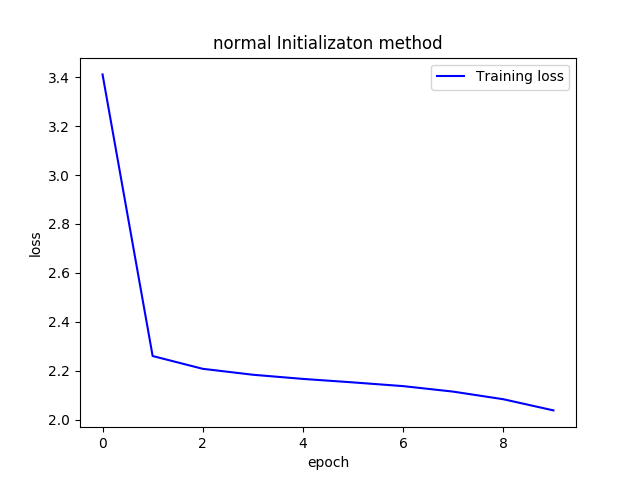
\includegraphics[width=0.7\textwidth]{normal_init.png}
\caption{\label{fig:init2}average loss against the training time (epoch) using normal initialization method.}
\end{figure}

\begin{figure}
\centering
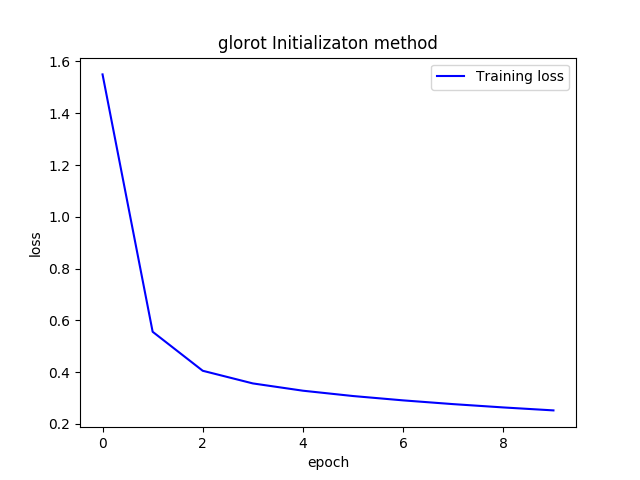
\includegraphics[width=0.7\textwidth]{glorot_init.png}
\caption{\label{fig:init3}average loss against the training time (epoch) using glorot initialization method.}
\end{figure}

\subsection{Hyperparameter Search}

\begin{enumerate}

\item
The combination of hyper-parameters that we found in which the average accuracy rate on the validation set reach 97.3\% accuracy:
Since we have the freedom to examine a variation of different architectures and hyperparameters, we chose a network with 2 hidden layers h1 (512 hidden units) and h2 (256 hidden units) with a total number of 535,818 parameters. We chose Relu activation, a learning rate of 0.01, a mini batch size of 64, the number of epochs as 30 and the glorot initialization. (See Figure \ref{fig:hyper}).

\item 
We tried different hyper-parameters for learning rate, different network architectures, batch sizes and activation functions (Tanh, Relu, Sigmoid).

\subsubsection{Changing the Learning rate}


\begin{itemize}

\item learning rate of 0.01: validation accuracy = 97.3\% (See Figure \ref{fig:hyper}).

\item learning rate of 0.1: validation accuracy = 98.1\% (See Figure \ref{fig:lr2}).

\item learning rate of 0.001: validation accuracy = 92.6\% (See Figure \ref{fig:lr3}).  
 
\item learning rate of 0.7: validation accuracy = 98.4\% (See Figure \ref{fig:lr4}). 
 
\end{itemize}

\begin{figure}
\centering
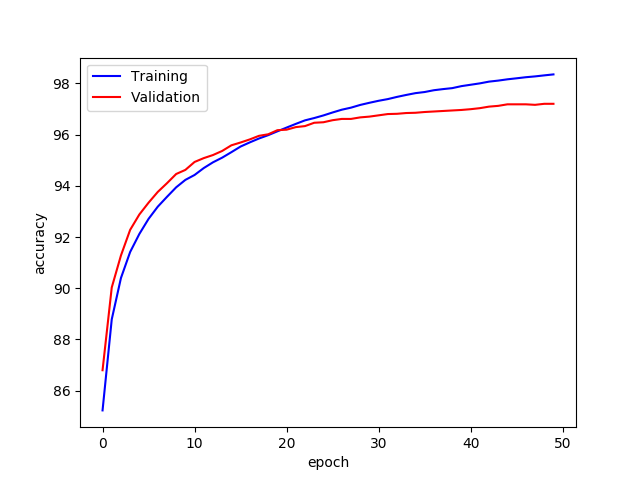
\includegraphics[width=0.7\textwidth]{acc_hyper.png}
\caption{\label{fig:hyper}Validation/training accuracy against the training time (epoch) using the chosen hyper-parameters.}
\end{figure}

\begin{figure}
\centering
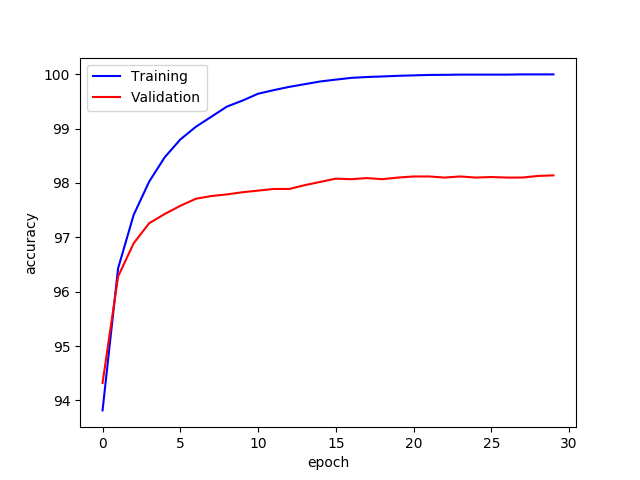
\includegraphics[width=0.7\textwidth]{lr2.png}
\caption{\label{fig:lr2}Validation accuracy against the training time (epoch) using a learning rate of 0.1.}
\end{figure}

\begin{figure}
\centering
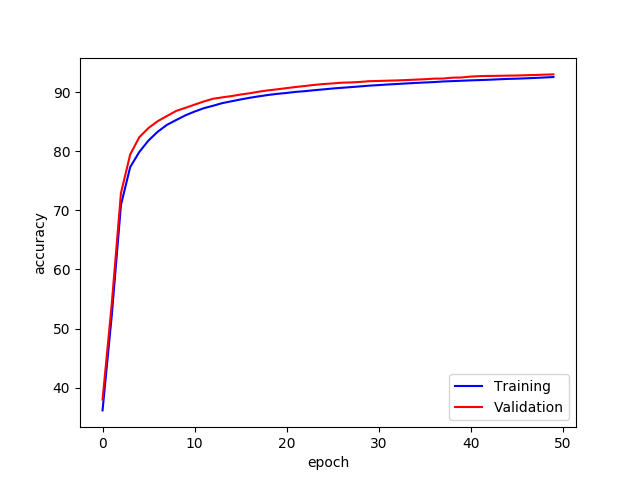
\includegraphics[width=0.7\textwidth]{lr3.png}
\caption{\label{fig:lr3}Validation accuracy against the training time (epoch) using a learning rate of 0.001.}
\end{figure}

\begin{figure}
	\centering
	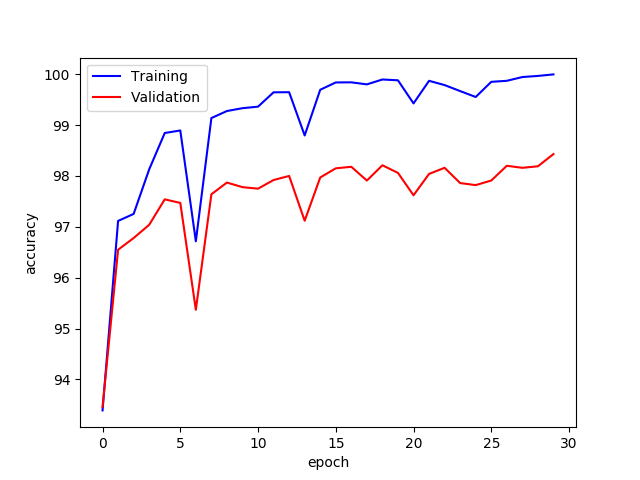
\includegraphics[width=0.7\textwidth]{lr4.png}
	\caption{\label{fig:lr4}Validation accuracy against the training time (epoch) using a learning rate of 0.7.}
\end{figure}

We observe that when the learning rate is low, training is more reliable, however, it takes much more time to converge. On the other hand, if the learning rate is high, then training may not converge and we observe unstable learning curve (since the weight changes is big and overshoot the local min).   

%We observe that when the learning rate is 0.1, the model overfits the training set while doing badly on the validation set. On the other hand, choosing a smaller learning rate (0.01) leads to a better performance on both training and validation sets i.e. not overfitting the training set while doing better on the validation set. 

%\subsubsection{Number of epochs}
%We keep the same settings and we only change the number of epochs.
%
%\begin{itemize}
%
%\item number of epochs of 50: validation accuracy = 97.2\% (See Figure \ref{fig:hyper}).
%
%\item number of epochs of 5: validation accuracy = 92.8\% (See Figure \ref{fig:epoch2}).
%
%\item number of epochs of 150: validation accuracy = 97.3\% (See Figure \ref{fig:epoch3}).  
%  
%\end{itemize}
%
%\begin{figure}
%\centering
%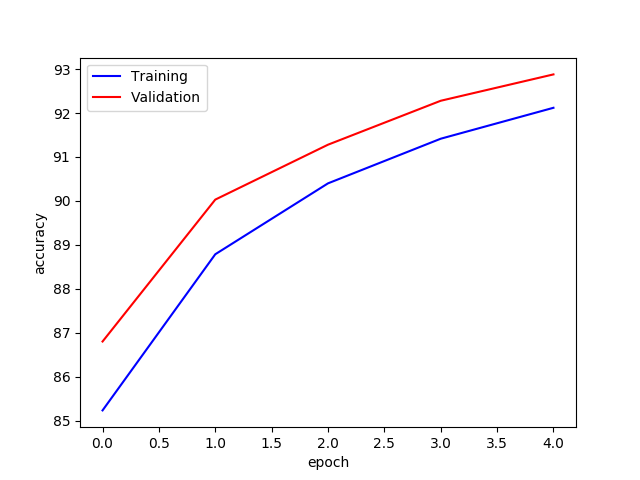
\includegraphics[width=0.7\textwidth]{epoch2.png}
%\caption{\label{fig:epoch2}Validation/training accuracy against the training time (epoch) using a number of epochs of 5..}
%\end{figure}
%
%\begin{figure}
%\centering
%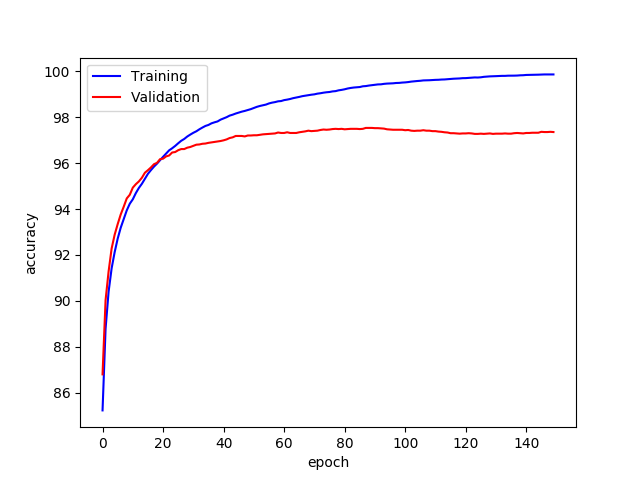
\includegraphics[width=0.7\textwidth]{epoch3.png}
%\caption{\label{fig:epoch3}Validation/training accuracy against the training time (epoch) using a number of epochs of 150.}
%\end{figure}

\subsubsection{Changing the Number of mini-batches}


\begin{itemize}

\item number of mini-batches of 64: validation accuracy = 97.3\% (See Figure \ref{fig:hyper}).

\item number of mini-batches of 8: validation accuracy = 97.4\% (See Figure \ref{fig:batch2}).

\item number of mini-batches of 512: validation accuracy = 93.1\% (See Figure \ref{fig:batch3}).  
  
\end{itemize}
We observe that the model performs better when the batch size is large.
\begin{figure}
\centering
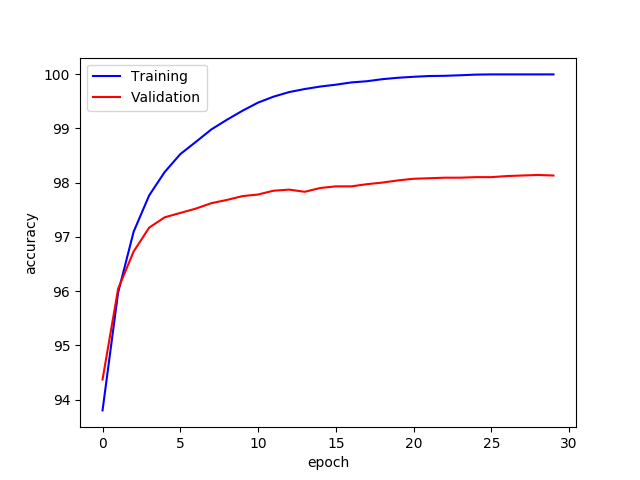
\includegraphics[width=0.7\textwidth]{batch2.png}
\caption{\label{fig:batch2}Validation/training accuracy against the training time (epoch) using a number of mini-batches of 8.}
\end{figure}

\begin{figure}
\centering
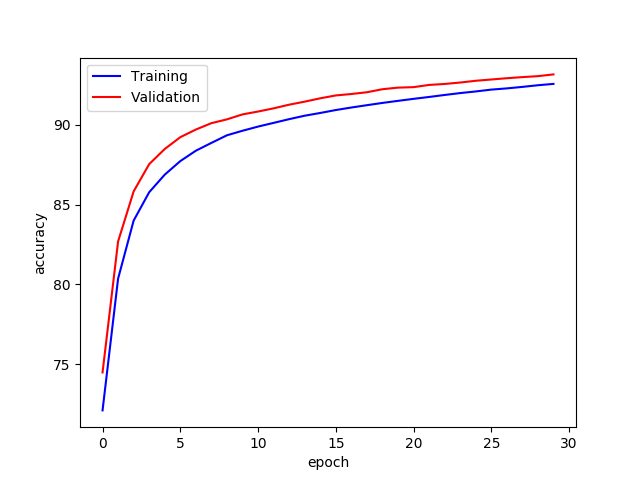
\includegraphics[width=0.7\textwidth]{batch3.png}
\caption{\label{fig:batch3}Validation/training accuracy against the training time (epoch) using a number of mini-batches of 512.}
\end{figure}

\subsubsection{Non-linearity activation function}


\begin{itemize}

\item Relu activation function: validation accuracy = 97.2\% (See Figure \ref{fig:hyper}).

\item Sigmoid activation function: validation accuracy = 92.2\% (See Figure \ref{fig:sigmoid}).

\item tanh activation function: validation accuracy = 93.9\% (See Figure \ref{fig:tanh}).  
  
\end{itemize}
Obviously Relu and tanh perform better in terms of accuracy. 
\begin{figure}
\centering
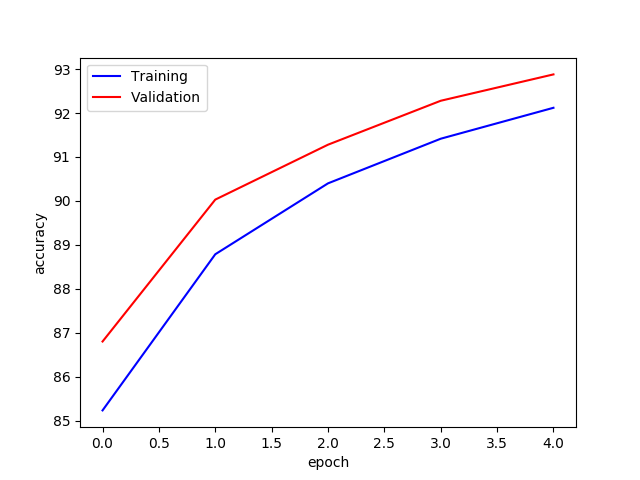
\includegraphics[width=0.7\textwidth]{epoch2.png}
\caption{\label{fig:sigmoid}Validation/training accuracy against the training time (epoch) using a sigmoid activation function.}
\end{figure}

\begin{figure}
\centering
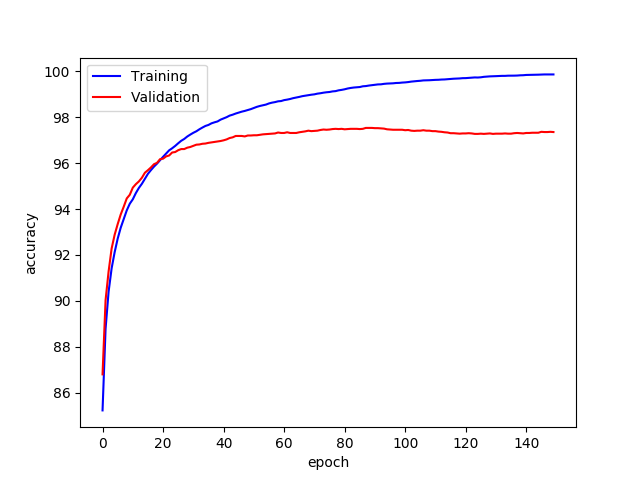
\includegraphics[width=0.7\textwidth]{epoch3.png}
\caption{\label{fig:tanh}Validation/training accuracy against the training time (epoch) using a tanh activation function.}
\end{figure}
\begin{figure}
	\centering
	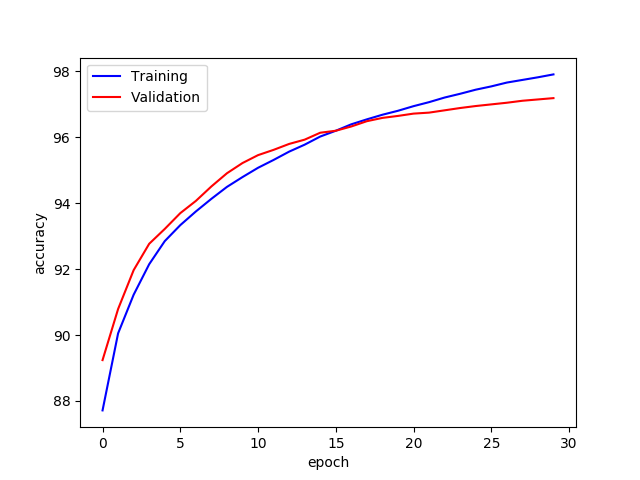
\includegraphics[width=0.7\textwidth]{arch2.png}
	\caption{\label{fig:arch2}Validation/training accuracy against the training time (epoch) using a network architecture with h1=32 and h2=64}
\end{figure}
\begin{figure}
	\centering
	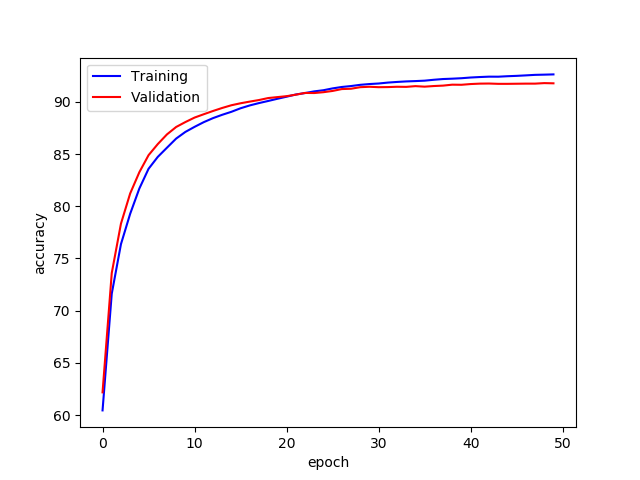
\includegraphics[width=0.7\textwidth]{arch3.png}
	\caption{\label{fig:arch3}Validation/training accuracy against the training time (epoch) using a network architecture with h1=10 and h2=5}
\end{figure}

\subsubsection{Network architecture (Chaning the number of hidden units)}


\begin{itemize}

\item Network with 2 hidden layers h1 = 64, h2 = 32: validation accuracy = 97.2\% (See Figure \ref{fig:hyper}).

\item Network with 2 hidden layers h1 = 32, h2 = 64: validation accuracy = 96.85\% (See Figure \ref{fig:arch2}).

\item Network with 2 hidden layers h1 = 10, h2 = 5: validation accuracy = 91.77\% (See Figure \ref{fig:arch3}).

\end{itemize}


\subsection{Gradient validation using finite difference approximation}
We implemented the gradient validation method \emph{grad\_check} under the mlp.py script which returns the maximum difference between the true gradient and the finite difference gradient approximation for a given precision $\epsilon$.

We validated the gradients for the first $p=\min(10,m)$ elements of the second layer weights ($W2$) with $m$ number of elements. Using $\epsilon=\frac{1}{N}$, Figure \ref{fig:grad_check} shows the maximum difference as a function of the $N$.

\begin{figure}
\centering
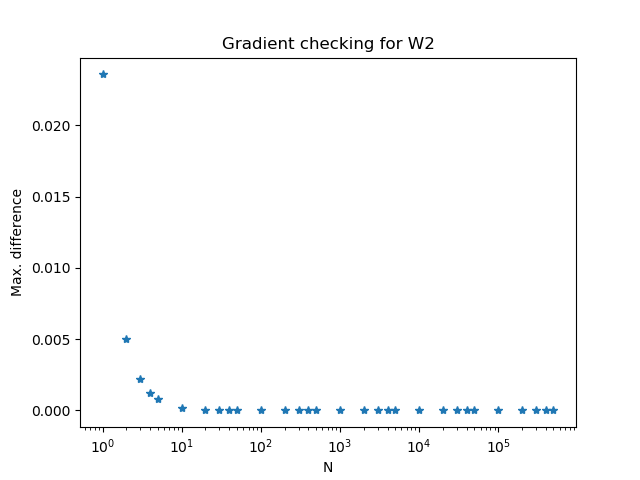
\includegraphics[width=0.7\textwidth]{grad_check}
\label{fig:grad_check}
\caption{Maximum difference between the analytic gradient and the finite difference approximation for some elements of the weight matrix at the second layer as a function of the precision $N = \frac{1}{\epsilon}$}
\end{figure}

The approximation of the gradient for each element gets closer to the real partial derivative as $\epsilon$ gets smaller, this is consistent with theory since in the definition of the derivative the epsilon tends to zero. 

\end{enumerate}

\section{Problem 2 Convolutional Networks}
\label{sec:problem2}
\subsection{Architecture}
As it is a common practice, we decided to implement our convolutional network using layers that sequentially apply a convolution followed by a ReLU followed by pooling.
Given the size of the images in the dataset MNIST ($28\times28$ pixels) we decided to use four layers where the convolutions are padded in order to keep the size and the pooling kernels have a spatial size $2\times2$ and stride of 2 to obtain a single spatial dimension at the end. In order to fix some other parameters we chose the convolution kernels to have the spatial size of $3\times3$ and the number of channels at to double at each convolution layer. With these settings the only parameter that controls the size of the network is the number of output channels at the first convolutional layer. 

In order to obtain a similar number of parameters than our mlp of Problem~\ref{sec:problem1} ($\sim50K$ parameters) we set that value to $12$, so the number of channels at the layers of our network are  $1,12,24,48,96$. 
\subsection{Performance}
Figure~\ref{fig:CNN_accuracy} shows the training and validation accuracy of the model at each epoch. After training the model for 10 epochs we obtain a validation accuracy of $98\%$

\begin{figure}[h!]
\centering
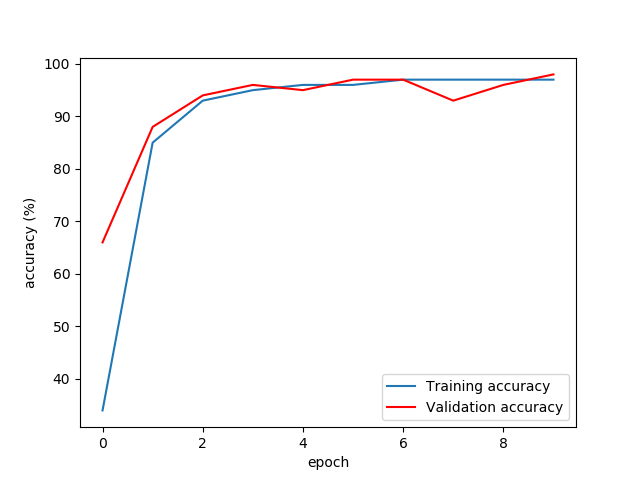
\includegraphics[width=0.7\textwidth]{P2_CNN_accuracySGD}
\label{fig:CNN_accuracy}
\caption{Training and validation accuracy of the convolutional model of Section~\ref{sec:problem2}}
\end{figure}

For similar number of parameters the CNN here performs better than the MLP in problem 1. Its accuracy is $98\%$ compared to $97.6\%$. This is an important improvement given that we did not perform hyperparameter tuning as in the case of MLP. Also, this CNN architecture is simple, compact and was designed with little manipulation.  

\newpage
\section{Problem 3 (Kaggle challenge)}
\label{sec:problem3}

\subsection{Architecture of the model}
The model's architecture that we have used is inspired from VGG model, which has the following components (see Figure \ref{fig:vgg}) :

\begin{itemize}
\setlength\itemsep{0em}
	\item[-] 13 convolutions layers, with 0 padding at each layer, and a kernel of size (3,3) and stride of 1.
	\item[-] The number of filters goes from 64 to 640 accross the layers
	\item[-] 5 max pooling with kernel of size (2,2) and stride of 2.
	\item[-] 2 fully connected layers with 4096 hidden units
	\item[-] 1 output layer
\end{itemize}

\begin{figure}[h!]
\centering
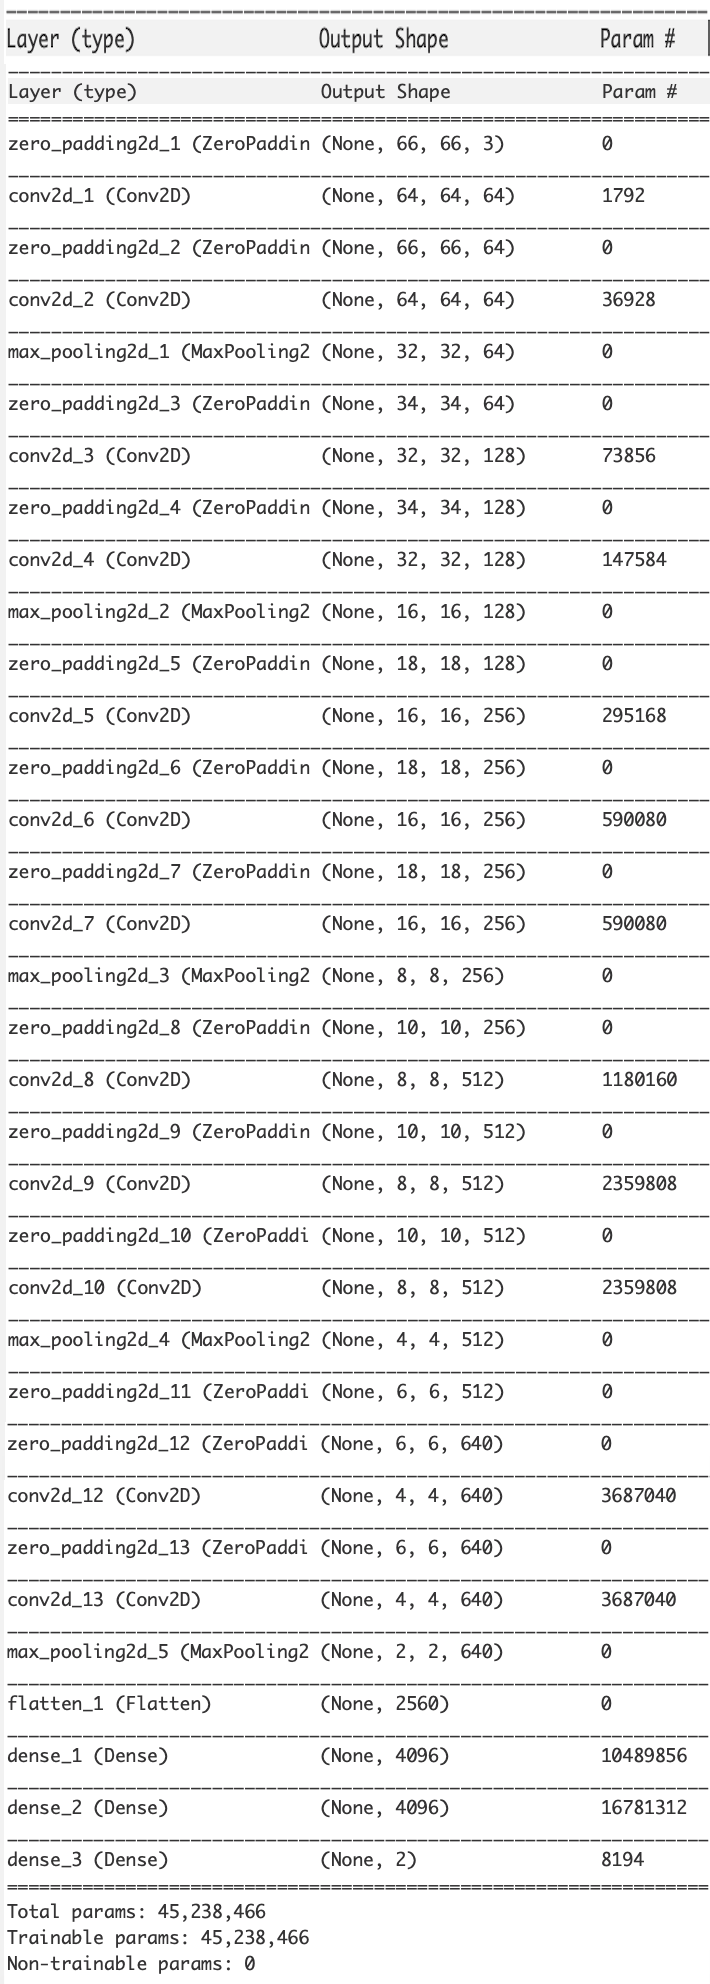
\includegraphics[scale=0.3]{VGG_arch.png}
\caption{Model architecture}
\label{fig:vgg}
\end{figure}

The total parameters of this model is $45,238,466$, which is a medium size in comparison with the most recent deep learning models.
%
Our experimentation has shown that a model with more layers performs better than a model with fewer ones. In fact, for this competition, we have found that the VGG model above have performed better than AlexNet-based architecture.

\subsection{Learning curves}
Figures \ref{fig:vggloss} and \ref{fig:vggacc} show respectively the training and validation loss and accuracy per epoch.
%
%
Before starting training the model, we have split the input images randomly to training and validation sets with a ratio of $80\%-20\%$ respectively. (see the code on appendix).
%
We have also used data augmentation strategy to improve the variance of the model. The transformation used were:
\begin{itemize}
\setlength\itemsep{0em}
\item[-]rescale by up to 1/255
\item[-]width shift by up to 0.2
\item[-]height shift by up to 0.2
\item[-]zoom by up to 0.5
\item[-]shear by up to 0.2,
\item[-]horizontal flip

\end{itemize}
%
The learning curves above show that the model reaches its optimal value around epoch 150. After that point, the model starts overfitting as the loss on validation set starts growing.
%
We believe that a regularization strategy as \textit{Weight decay} could potentially get a better result, as it will push the model to learn beyond 150 epochs without overfitting.
%
Notice that the accuracy on the test set is better than the accuracy on the validation set, which is a proof that the model generalize well, and the data augmentation strategy did well to improve the model's performance.

\begin{figure}[h!]
	\centering
	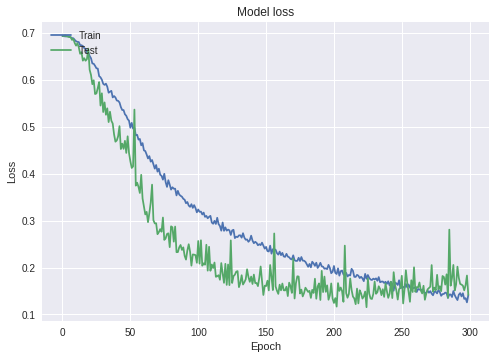
\includegraphics[scale=.6]{VGGLoss_of2.png}
	\caption{Loss of the model by epoch}
	\label{fig:vggloss}
\end{figure}

\begin{figure}[h!]
	\centering
	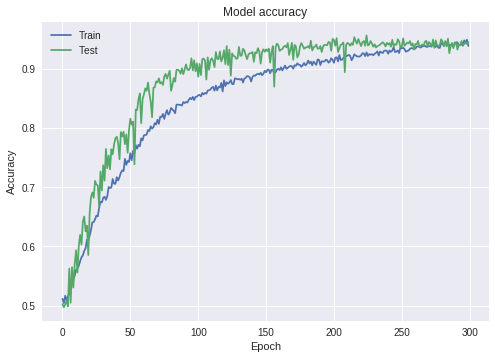
\includegraphics[scale=.6]{VGGAccu_of2.png}
	\caption{Accuracy of the model by epoch}
	\label{fig:vggacc}
\end{figure}

\newpage
\subsection{Hyperparameters settings}
In order to get a better performance, we have to choose the most relevent values for the hyperparameters during validation phase. That is, computing the accuracy and the loss of the model on validation set for multiple values of these hyperparameters. The hyperparameters that we have decided to tune are:
\begin{itemize}
\setlength\itemsep{0em}
\item[-]Number of hidden layers
\item[-]Size of the kernels
\item[-]Learning rate
\item[-]Batch size
\end{itemize}
%
We will give for each of these hyperparameters the accuracy and the loss of the model while keeping the others fixed.
%
The Table~\ref{table:1} shows the performance of the model with different number of convolutional layers.
%
\begin{table}[h!]
	\centering
	\begin{tabular}{||c c c c||} 
		\hline
		Nbr of layers & Accuracy & Loss & Total nb of parameters\\ [0.5ex] 
		\hline\hline
		6 & 0.3109 & 0.8574 & 2,736,066\\ 
		10 & 0.2713 & 0.8841 & 5,147,458\\ 
		13 & 0.2068 & 0.9078 & 17,076,546\\ 
		16 & 0.9445 & ? & 23,111,490\\
		19 & 0.9304 & 0.1922 & 39,896,898\\  [1ex] 
		\hline
	\end{tabular}
	\caption{Number of layers tuning}
	\label{table:1}
\end{table}
%
We notice that a model has a better performance when it has more hidden layers. This is normal because more layers means bigger capacity for the model. But this is not leanier, that is a deeper model is more likely to overfit if there is no regularization. That is what we have noticed with VGG with 19 layers.
%
The next Table~\ref{table:2} gives a comparison of the model's performance using different kernel sizes. This hyperparameter influence drastically the architecture of the model, that is a bigger kernel shorten the depth of the model and it could not be deeper unless we add 0 padding. We notice that in general a smaller kernel size gives a better result!

\begin{table}[h!]
	\centering
	\begin{tabular}{||c c c||} 
		\hline
		Kernel size & Accuracy & Loss \\ [0.5ex] 
		\hline\hline
		2 & 0.5832 & 0.6919 \\ 
		3 & 0.5761 & 0.6912 \\ 
		4 & 0.5444 & 0.6894 \\ 
		5 & 0.5418 & 0.6930 \\ [1ex]  
		\hline
	\end{tabular}
	\caption{Kernel size tuning}
	\label{table:2}
\end{table}

Table~\ref{table:3} gives a comparison of the model's performance as a function of the batch size. We notice that a small batch size push the model to make more iterations, and thus the SGD has a bigger chance to converge with enough epochs. Wheras, with a larger batch size, the SGD makes less iteration and may not get its minima within the same number of epochs.
%
\begin{table}[h!]
	\centering
	\begin{tabular}{||c c c||} 
		\hline
		Batch size & Accuracy & Loss \\ [0.5ex] 
		\hline\hline
		16 & 0.5320 & 0.6892 \\ 
		32 & 0.5015 & 0.6919 \\ 
		64 & 0.4859 & 0.6935 \\ 
		128 & 0.5000 & 0.6929 \\ [1ex]  
		\hline
	\end{tabular}
	\caption{Kernel size tuning}
	\label{table:3}
\end{table}

And finally, Table~\ref{table:4} gives a comparison of the model's performance as a function of the learning rate. We notice, that the model converges slowly with a small learning rate and faster with a relatively bigger one like 0.03.

\begin{table}[h!]
	\centering
	\begin{tabular}{||c c c||} 
		\hline
		Learning rate & Accuracy & Loss \\ [0.5ex] 
		\hline\hline
		0.03 & 0.8935 & 0.2417 \\ 
		0.01 & 0.8595 & 0.3279 \\ 
		0.003 & 0.6930 & 0.5981 \\
		0.001 & 0.5825 & 0.6709 \\ [1ex]  
		\hline
	\end{tabular}
	\caption{Kernel size tuning}
	\label{table:4}
\end{table}

According to our hyperparameter search, we set the final model as follows:
\begin{itemize}
\setlength\itemsep{0em}
\item[-]Number of hidden layers: 13 convolutions and 3 FC
\item[-]Size of the kernels: (3,3)
\item[-]Learning rate: 0.015
\item[-]Batch size: 16
\item[-]Number of epochs: 300
\end{itemize}
%
This model give an accuracy of : $95\%$ on validation set and $94\%$ on the public leaderboard (see Figure \ref{fig:kaggle}). The model was trained for 200 epochs but get its best parameters around 150 epochs.
%
As we haven't used any regularization strategies, on the training phase, we have used the early stopping strategy, that is taking the best model's parameters before it starts overfitting.

\begin{figure}[h!]
	\centering
	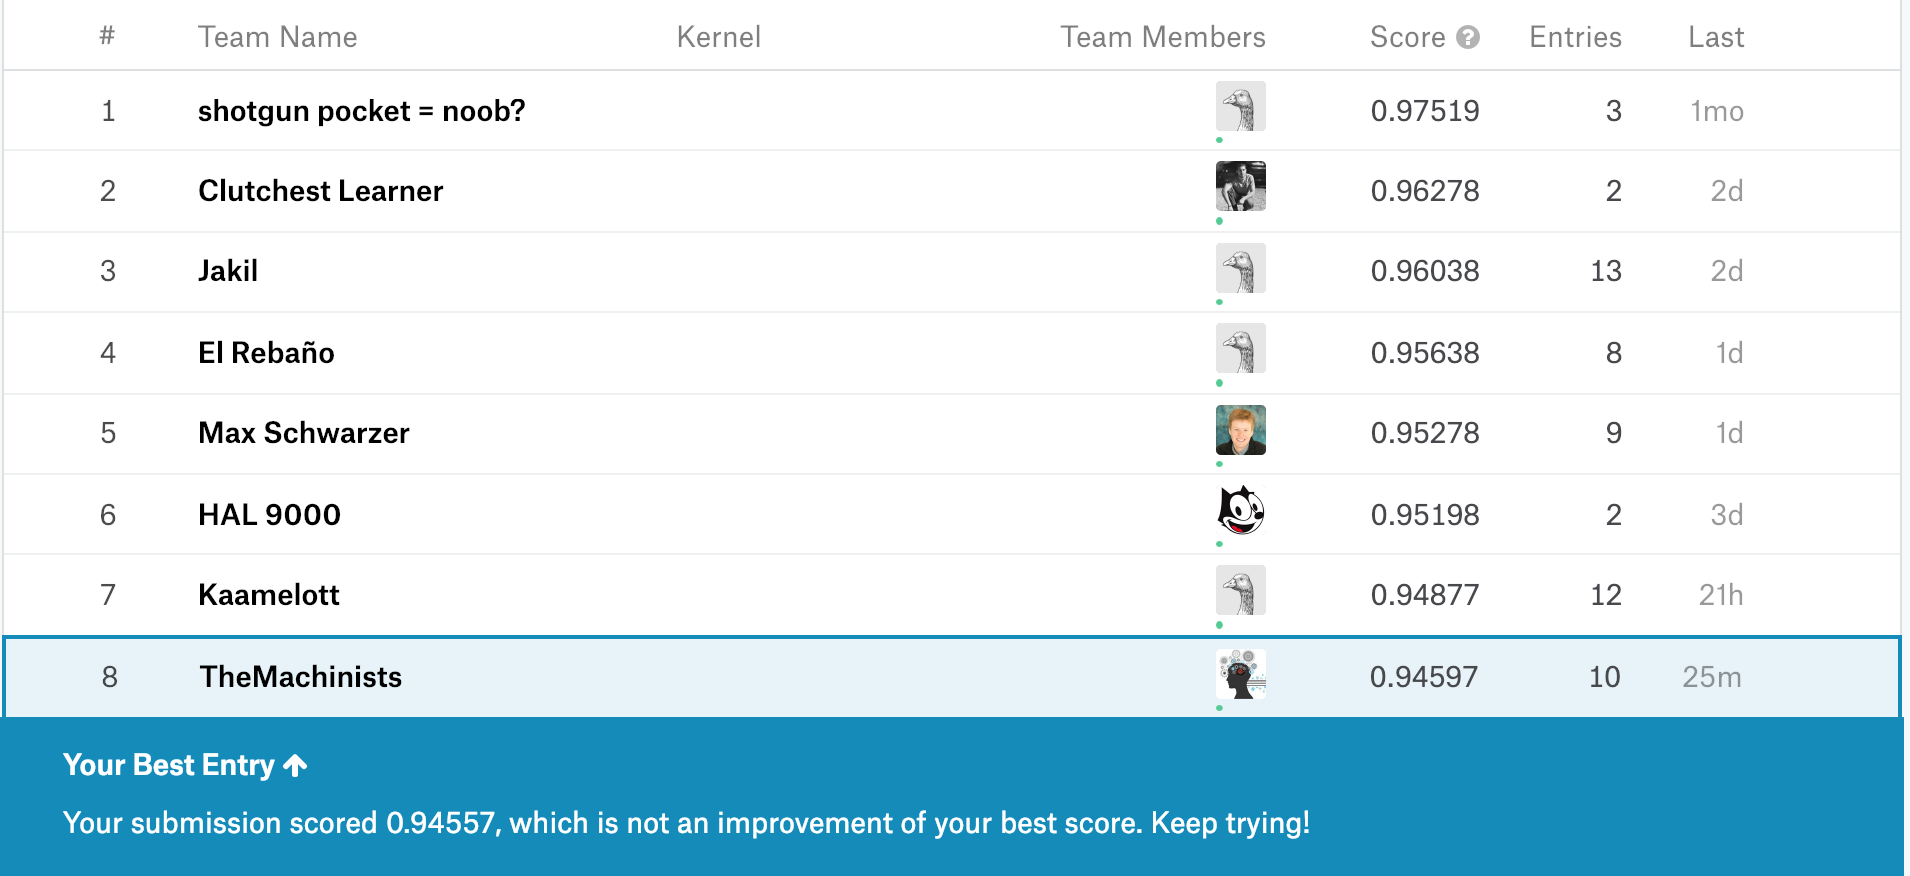
\includegraphics[scale=.4]{kaggle.png}
	\caption{Rank at the public leaderboard}
	\label{fig:kaggle}
\end{figure}

\subsubsection{Feature map visualization}
The feature map visualization gives in some sens an intuition on how a CNN learns from images. Across the layers, feature map go from high level pattern to low level as we go deeper in the model. The following image shows for each layers the feature map after each activation layer. The code used to display these images was taken from the blog \cite{featuremap}.

\begin{figure}[h!]
	\centering
	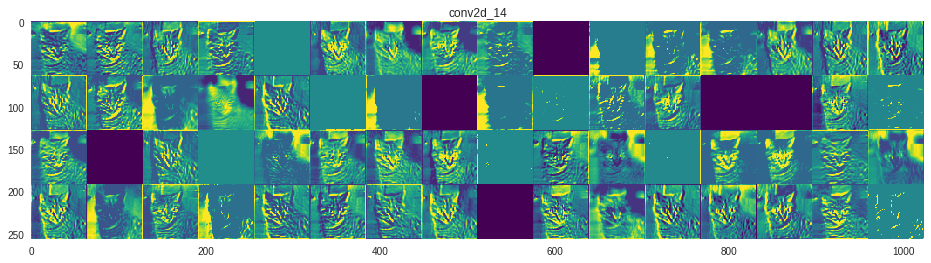
\includegraphics[scale=.3]{fp1.png}
	\caption{Feature map after conv layer 1}
	\label{fig:fp1}
\end{figure}

\begin{figure}[h!]
	\centering
	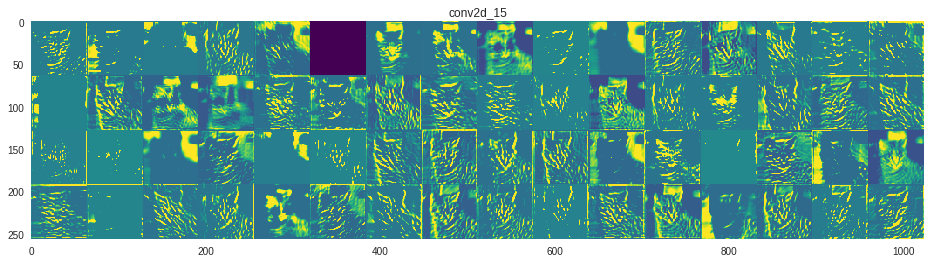
\includegraphics[scale=.3]{fp2.png}
	\caption{Feature map after conv layer 2}
	\label{fig:fp2}
\end{figure}

\begin{figure}[h!]
	\centering
	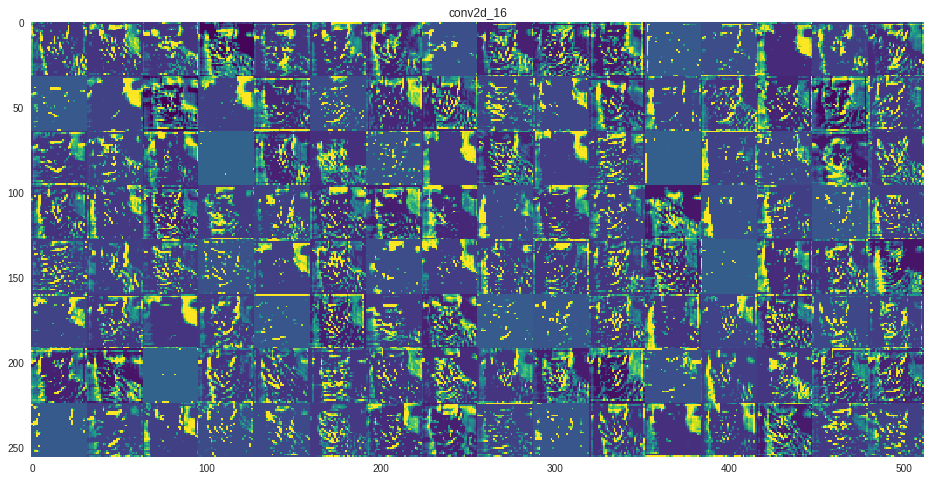
\includegraphics[scale=.3]{fp3.png}
	\caption{Feature map after conv layer 3}
	\label{fig:fp3}
\end{figure}

\subsubsection{Performance of the model}
The model gets $94\%$ accuracy on test set (public leaderboard) which is not bad given that we haven't used any fancy techniques like regularization. It is interesting to investigate which images the model has misclassified, in order to identify ways to improve the model's performance. 

To understand why the model has done such misclassification, we will display a sample of two kind of mislcassifications:

\begin{itemize}
	\item[(a)] The model clearly misclassified images:\\
	In the Figure \ref{fig:100misclass}, we can see a sample of images that the model has misclassified with probability $>= 0.6$.
	We notice that these images are noisy and doesn't show clearly the animal's figure or they contains other objects like human or fences.
	%
	\begin{figure}[h!]
		\centering
		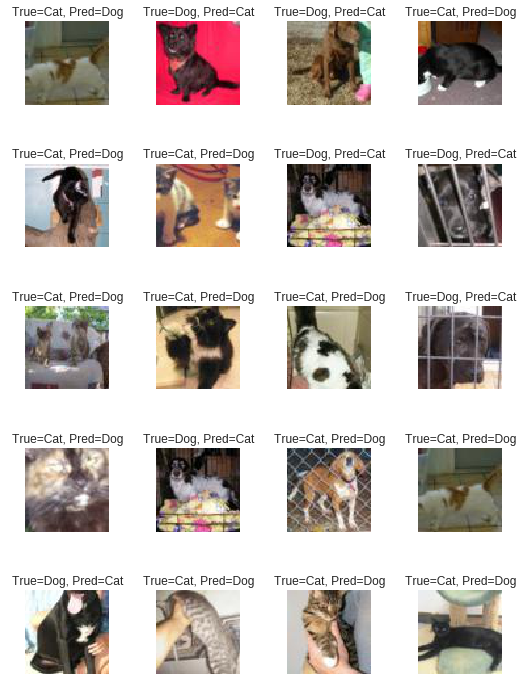
\includegraphics[scale=.36]{100misclass.png}
		\caption{100\% miclassification}
		\label{fig:100misclass}
	\end{figure}
%
\begin{figure}[h!]
	\centering
	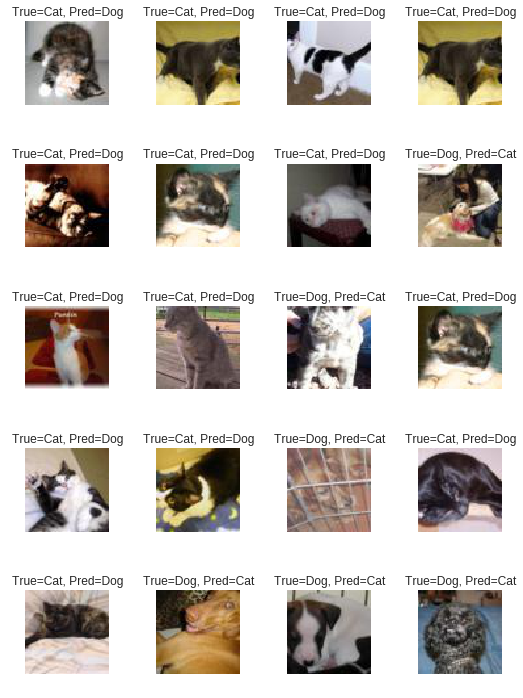
\includegraphics[scale=.36]{50misclass.png}
	\caption{Around 50\% miclassification}
	\label{fig:50misclass}
\end{figure}
%
\item[(b)] The model predicts around $50\%$ on both classes:\\
In the Figure \ref{fig:50misclass} we can see some images that the model have bearly misclassified them. We notice the same pattern as the item (a) where the animals took different position in the picture with other objects or half captured.
%
\end{itemize}
%
As a conclusion, the classifier that we have build was able to classify correctly $94\%$ of images which is a good result without even using any regularization or fancy optimization algorithm. However, the model couldn't classify some images because of it's complexity, like having other objects around or taking just a part of the animal. In that case, we may suggest to add more data by sampling over those kind of misclassified images and give train the model on them, or use the K-Fold cross validation in order to train the model on all kind of images.
 
 \newpage
\begin{thebibliography}{9}
\bibitem{weights} 
  Jayadevan Thayumanav: Why don't we initialize the weights of a neural network to zero?, 2018.
  \\\texttt{https://www.quora.com/Why-dont-we-initialize-the-weights-of-a-neural-network-to-zero}
  \bibitem{featuremap} 
  Applied Deep Learning - Part 4: Convolutional Neural Networks
  \\\texttt{https://towardsdatascience.com/applied-deep-learning-part-4-convolutional-neural-networks-584bc134c1e2}
    \bibitem{github} 
  TheMachinists github repository: Representation-Learning
  \\\texttt{https://github.com/faresbs/Representation-Learning.git}
\end{thebibliography}
\end{document}